%Esto es un comentario :D 
%------------------Encabezado: tiene los paquetes----------------------------------
%Empezamos definiendo que tipo de documento vamos a usar.
%respetar la gerarquía entre corchetes y llaves. Paquetes y especifidad.

\documentclass[onecolumn]{article} %report, book %números de columnos
\usepackage[spanish]{babel} %Para las cosas en español (referencias, etc) Babel puede tener problemas.
%Renombrar los comandos.
\usepackage[latin1,utf8]{inputenc} %idioma, latin1:español, inputenc es el paquete de idiomas de occidente %utf8, guión, comas, mayor que, etc, lo que se puede teclar.
\usepackage{graphics,graphicx,xcolor} %xcolor, para colores %figuras
\usepackage{amssymb,amsmath} %Lenguaje matemático %amsmath, el de las integrales
\usepackage{verbatim} %Escribir código
\usepackage{bm} %negrita
%Cambiar margenes, usar más paquetes.
%Fecha en español. Nota: \renewcommand. También paquete para email.
%C y C++, Funciona de manera similar, con paquetes, primero los introducimos.
%Como escribir el simbolo porcentaje sin añadir comentario
%Reducir tamaño de margenes
%Cambiar fuente de letra, tamaño de letra, centrar, alinear a la izquierda, cambiar el temmplate. "centrar section latex"
%Como poner las comillas en español
%Cambiar simbolo de la viñeta

%---------------------------------------------------------------------
\title{Mi primer proyecto en Overleaf, Tercera clase}
\author{CARLOS ANDRES RODALLEGA MILLAN}
\date{\today}

%---------------------------------------------------------------------
%Toda pareja que comienza con \Begin y termina con \END se llama ENTORNO
%++++++++++++++++++++++CUERPO DEL DOCUMENTO+++++++++++++++++++++++++++
\begin{document}
\maketitle %HAGA el título.... (que está arriba)
%.-.-.-.-.
\section{Inclusión de texto} %Hace una sección
Si yo comienzo a escribir en mi documento, me doy cuenta que simplemente el texto comienza a ser parte de mi documento.
\subsection{Enumeraciones: con números o con viñetas}
Comencemos con la enumeraciones que utilizan números para cada uno de los ítems.
%enumeraciones con números
\begin{enumerate}
    \item Recuerde que toda pareja que comienza "begin" y termina con "end" se llama ENTORNO
    \item Las secciones no son entornos.
\end{enumerate}
%Tabular para saber que es lo que está dentro del entorno. %Se respeta la jerarquía.
También puedo tener entornos que enumeran con viñetas.
\begin{itemize}
    \item Primera viñeta.
    \begin{enumerate}
        \item Primer número.
        Intalen el Texmaker para   
        \begin{itemize}
            \item Esta es la primera viñeta de la primera enumeración de la primera viñeta
        \end{itemize}
        \item Segundo número.
    \end{enumerate}
    \item Segunda viñeta.
    \item La tercera viñeta.
\end{itemize}
\section{Inclusión de ecuaciones} %Hace una sección
Haremos ina introducción a la escritura de ecuaciones usando LaTex, como herramienta principal de comunicación en la realización de documentos científicos
	\subsection{Ecuaciones de una sola línea}
	Haremos primero un ejemplo de ecuación sin enumeración y que se encuentra en una línea:
	%Signo pesos doble
	$$y(t)=y_0+v_0+\frac{1}{2}at^2$$
	Si queremos colocar un conjunto de subíndices lo que debemos hacer es colocarlos todos o agruparlos entre 				corchetes. \{\}

	%Así se puede colocar cosas entre corchetes
	$$x_{0,1}=f(x_{2,1},x_{4,3})$$
	Para escribir ecuaciones que sí tengan enumeración entonces usamos el entorno \verb+equiation+
	%como meter código entre línea con una forma diferente.
	%El nombre siempre se guarda en el archivo auxiliar. (50 ecuaciones).
	%Compilar dos veces.
\begin{equation}
	\label{ec_mov y} %Sirve para dar el nombre
	y(t)=y_0+v_0+\frac{1}{2}at^2
\end{equation}
Para obtener esta ecuación \ref{ec_mov y}, usamos el siguiente código que esta escrito mediante el entorno \verb+verbatim+:
	\begin{verbatim}
		\begin{equation}
		y(t)=y_0+v_0+\frac{1}{2}at^2
		\end{equation}
	\end{verbatim}
La pareja \verb+label+ y \verb+ref+ es la que se utiliza para darle nombres a una ecuación, figura, tabla, etc, y luego llamarla en el texto.
	\subsection{Ecuaciones de más de una línea}
	Para escribir ecuaciones de una línea vamos a usar el entorno \verb+eqnarray+ o el entorno \verb+align+ 
\paragraph{Veamos dos ejemplos:}
Escribamos tres de las hermosas ecuaciones de Maxwell
\begin{eqnarray}
	\label{Max3}
	\nabla\cdot\mathbf{E} &=&\rho \nonumber\\
	\nabla\cdot\mathbf{B} &=&0. \\
	\nabla\times\mathbf{E} &=& \mathbf J \nonumber
%Signo & es indispensable el uso de este uso de estas alineaciones.
%\nonumber sirve para no dejar la enumeración. Todo el conjunto se llama dos.
\end{eqnarray}
En el \verb+eqnarray+ es indispensable el uso del \& a lado y lado del símbolo por el que vamos a alinear las ecuaciones como se muestra en la ecuación \ref{Max3}
{\bf Nota: no olvidar cortar las línea usando un doble backslash, la última línea no se corta}
\\
La otra forma es usando el entorno \verb+align+
\begin{align}
f(x)&=\alpha + \beta x + \gamma x^2 \nonumber \\ 
&+\delta x^3  \\
&+\rho x^4+ \lambda x^5 \nonumber
\end{align}
%Ver el uso de &
Para omitir la enumeraciones de cualquiera de los entornos, bastan con colocar un * en el lado derecho del entorno.
\begin{align*}
f(x)&=\alpha + \beta x + \gamma x^2 \\ 
&+\delta x^3  \\
&+\rho x^4+ \lambda x^5 
\end{align*}
\subsection{Ecuaciones embebidas en el texto}
También es posible colocar ecuaciones entre el texto. Por ejemplo, si yo hablo de la ecuación de la recta, la cual tiene la forma funcional $y=mx+b$.Puedo escribirla usando un único símbolo \$ antes y después de la ecuación.


\section{Inclusión de gráficas} %Hace una sección
%Insertaremos las graficas de gnuplot.
La gráfica la incluimos en LaTex, usando el entorno \verb+figure+ con el comando \verb+includegraphics+
\begin{figure}[h!]%[h! here, para la gráfica]
	\centering %para centrar
	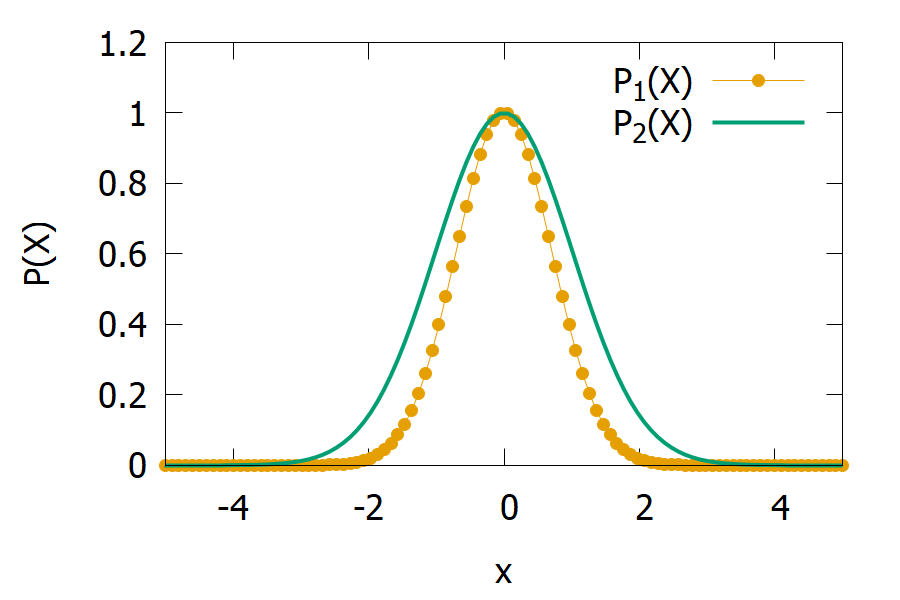
\includegraphics[scale=0.2]{Grafica26Nov.png}
	\caption{\label{fig_exp}Es una gráfica que contiene dos curvas de funciones Gaussianas, una con líneas y puntos y 		la otra con solo línea} %Enumera la gráfica.
	%Tarea, como cambiar a español.
\end{figure}
\begin{figure}[h!]%[h! here, para la gráfica]
	\centering %para centrar
	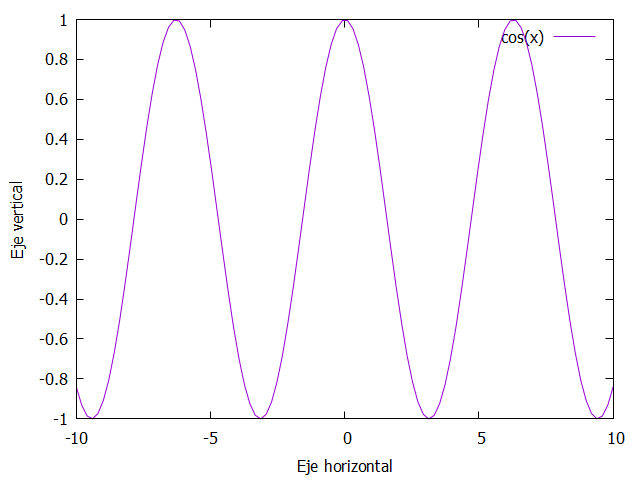
\includegraphics[scale=0.2]{grafica_16Nov.png}
	\caption{\label{fig_cos}Es una gráfica que contiene la figura coseno.} %Enumera la gráfica.
	%Tarea, como cambiar a español.
\end{figure}

\newpage %mandamos a una página nueva.

\section{Inclusión de tablas} %Hace una sección
%Para las tabla tenemos, table y tabular
Vamos hoy a hacer tablas \cite{normal}, existen dos dos entornos que son los realmente importantes:
\begin{enumerate}
	\item El entorno \verb+Tabular+: realmente ayuda a la realización de la tabla. %Especifica a los items de la 			tabla.
	\item El entorno \verb+Table+: ayuda a incluir el \verb+caption+(Descripción de la tabla, enumeración, etc), 			también ayuda con \verb+centering+. %Hace la tabla
\end{enumerate}
Podemos hacer el uso de estos dos entornos para crear la \ref{Tabla_primera}.
	\begin{table}[h!] %h! es una orden, here h, top t, bottom b, se puede combinar la prioridad [thb]
	\centering
	%Las llaves es para información al lado derecho, la información de las columnas
		\begin{tabular}{|l|c|r|}%Información columnas (Alineada, centrada, etc, lcr)
		\hline
		Columna 1 & Columna 2 & Columna 3 \\ \hline%3 elementos, seprados
		Izquierda & Está centrada & Derecha\\
		\hline
		$\Psi(x)=\hat{H}\psi$ & $\int_a^b f(x)dx$ & $\frac{\partial g}{\partial x}= h(x)$ \\
		\hline
		\end{tabular}
	\caption{\label{Tabla_primera} Esta es el caption de aprender a hacer tablas xd}
	\end{table}
\begin{align*}
z&= x  & a&=z  & b&=a+c  \\ 
zsada&= x  & adsds&=z  & bgfgf&=a+c\\
zdsd&= x  & adsdf&=z  & bgfs&=a+c  \\
zdsd&= x  & adsdf&=z  & bgfs&=a+c\\
\end{align*}


	
\begin{thebibliography}{99} %Bibliografia, información que tenemos en nuestras referencias %bibitem
\bibitem{normal} Apellido1, Nombre1, Nombre de la Revista, Vol., página(año). 

\end{thebibliography}
\end{document}
